


\begin{figure}[ht]
	\centerline{
\includegraphics[width=0.60\textwidth]{Gambar/dapi7.jpg}}
	\caption{File I/O}
	\label{File I/O}
\end{figure}



\section {Pengertian }
\subsection {Python File I/O}

Unit~input~adalah (masukan) suatu  data yang berbentuk documet bait itu data data foto, data data hurup ataupun data tanggal ke dalam sebuah system yang  terkomputerisasi.  unit output (keluaran) biasanya digunakan untuk menampilkan data, atau dengan kata lain untuk menangkap data yang telah diinputkan terlebih dahulu dalam sebuah penyimpanan media elektronic , contohnya data yang akan ditampilkan pada layar monitor atau printer. \par
I/O Input/Ouput Read [IOR] dan untuk tulis I/O Input/Output Write [IOW]. File adalah lokasi bernama pada disk untuk menyimpan informasi terkait. Ini digunakan untuk menyimpan data secara permanen dalam memori non-volatile (misalnya hard disk). Karena, random access memory (RAM) bersifat volatile sehingga kehilangan datanya saat komputer dimatikan, kita menggunakan file untuk penggunaan data masa depan. Bila kita ingin membaca dari atau menulis ke file kita perlu membukanya terlebih dahulu. Bila sudah selesai, perlu ditutup, agar sumber yang diikat dengan file tersebut dibebaskan.Oleh karena itu, dengan Python, sebuah operasi file berlangsung dengan urutan sebagai berikut. \par
\vspace{12pt}
\noindent 

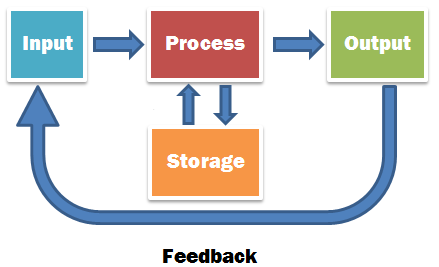
\includegraphics[width=15cm,height=7cm]{Gambar/dapi8.jpg}
\begin{equation}Python File I/O\end{equation}


\begin{enumerate}
	


	\item Buka file 

	\item Membaca atau menulis (melakukan operasi) 
	\item Tutup file tersebu 
	\end {enumerate}
\vspace{12pt}
\vspace{12pt}
\vspace{12pt}
\noindent 
Membuka sebuah file \par
\noindent 
Python memiliki built-in function open () untuk membuka file. Fungsi ini mengembalikan objek file, juga disebut handle, karena digunakan untuk membaca atau memodifikasi file yang sesuai. \par
\vspace{12pt}
\noindent 

\begin{verbatim}

>>>~f~=~open("test.txt")    
 $  \#  $ open file in current directory \par
\noindent 
>>>~f = open("C:/Python33/README.txt")  
 $  \#  $ specifying full path \par
\vspace{12pt}

\end{verbatim}

Kita bisa menentukan mode saat membuka file. Dalam mode, kami menentukan apakah kita ingin membaca 'r', menulis 'w' atau menambahkan 'a' ke file. Kita juga menentukan apakah kita ingin membuka file dalam mode teks atau mode biner. Defaultnya adalah membaca dalam mode teks. Dalam mode ini, kita mendapatkan string saat membaca dari file. Di sisi lain, mode biner mengembalikan byte dan ini adalah mode yang akan digunakan saat berhadapan dengan file non-teks seperti file gambar atau exe. \par
\vspace{12pt}
\vspace{12pt}
\noindent 

\begin{enumerate}


\item 'r' \hspace*{0.5in}  \par
\noindent 
Buka file untuk dibaca. (default) \par
\vspace{12pt}
\noindent 

\item 'w' \hspace*{0.5in}  \par
\noindent 
Buka file untuk menulis. Membuat file baru jika tidak ada atau memotong file jika file tersebut ada. \par
\vspace{12pt}
\noindent 

\item 'x' \hspace*{0.5in}  \par
\noindent 
Buka file untuk pembuatan eksklusif. Jika file sudah ada, operasi gagal \par
\vspace{12pt}
\noindent 

\item 'a' \hspace*{0.5in}  \par
\noindent 
Buka untuk menambahkan di akhir file tanpa memotongnya. Membuat file baru jika tidak ada. \par
\vspace{12pt}
\noindent 

\item 't' \hspace*{0.5in}  \par
\noindent 
Buka dalam mode teks. (default) \par
\vspace{12pt}
\noindent 

\item 'b' \par
\noindent 
Buka dalam mode biner. \par
\vspace{12pt}
\noindent 
\item '+' \par
\noindent 
Buka file untuk mengupdate (membaca dan menulis) \par
\vspace{12pt}
\noindent 

\end {enumerate}

\begin{verbatim}

f~=~open("test.txt")~~~   
 $  \#  $ equivalent to 'r' or 'rt' \par
\noindent 
f~= open("test.txt",'w')  
 $  \#  $ write in text mode \par
\noindent 
f = open("img.bmp",'r+b') 
 $  \#  $ read and write in binary mode \par
\vspace{12pt}
\noindent 

\end{verbatim}

Tidak seperti bahasa lain, karakter 'a' tidak menyiratkan angka 97 sampai dikodekan menggunakan ASCII (atau pengkodean setara lainnya). Apalagi, pengkodean default bergantung pada platform. Di jendela, itu adalah 'cp1252' tapi 'utf-8' di Linux. Jadi, kita juga tidak harus bergantung pada pengkodean default atau kode kita akan berperilaku berbeda di berbagai platform. Oleh karena itu, ketika bekerja dengan file dalam mode teks, sangat disarankan untuk menentukan jenis pengkodean. \par
\vspace{12pt}
\noindent 
f = open("test.txt",mode = 'r',encoding = 'utf-8') \par
\vspace{12pt}
\noindent 
\section{Menutup sebuah File}
Ketika kita selesai dengan operasi ke file, kita perlu menutupinya dengan benar. Menutup file akan membebaskan sumber daya yang terkait dengan file dan dilakukan dengan menggunakan metode close (). Python memiliki pengumpul sampah untuk membersihkan benda yang tidak difermentasi tapi, kita tidak boleh bergantung padanya untuk menutup file. \par
\noindent 
f = open("test.txt",encoding = 'utf-8') \par
\noindent 
$  \#  $ perform file operations \par
\noindent 
f.close() \par
\vspace{12pt}
\noindent 
Metode ini tidak sepenuhnya aman. Jika pengecualian terjadi saat kita melakukan operasi dengan file, kode keluar tanpa menutup file. Cara yang lebih aman adalah dengan menggunakan try ... akhirnya blok. \par
\vspace{12pt}
\noindent 
try: \par
\noindent 
~~ f = open("test.txt",encoding = 'utf-8') \par
\noindent 
~~  $  \#  $ perform file operations \par
\noindent 
finally: \par
\noindent 
~~ f.close() \par
\vspace{12pt}
Dengan cara ini, kita dijamin bahwa file tersebut benar tertutup bahkan jika pengecualian dinaikkan, menyebabkan aliran program berhenti. Cara terbaik untuk melakukannya adalah dengan menggunakan pernyataan. Ini memastikan file ditutup saat blok di dalam dengan keluar. Kita tidak perlu secara eksplisit memanggil metode close (). Hal itu dilakukan secara internal. \par
\vspace{12pt}
\noindent 
with open("test.txt",encoding = 'utf-8') as f: \par
\noindent 
~~  $  \#  $ perform file operations \par
\vspace{12pt}
\noindent 
\section{Menulis ke File}
Untuk menulis ke file kita perlu membukanya dalam mode write 'w', tambahkan 'a' atau exclusive creation 'x'. Kita harus berhati-hati dengan mode 'w' karena akan menimpa file jika sudah ada. Semua data sebelumnya terhapus. Menulis string atau urutan byte (untuk file biner) dilakukan dengan menggunakan metode write (). Metode ini mengembalikan jumlah karakter yang ditulis ke file. \par
\vspace{12pt}
\noindent 
with open("test.txt",'w',encoding = 'utf-8') as f: \par
\noindent 
~~ f.write("my first file $  \setminus  $n") \par
\noindent 
~~ f.write("This file $  \setminus  $n $  \setminus  $n") \par
\noindent 
~~ f.write("contains three lines $  \setminus  $n") \par
\vspace{12pt}
Program ini akan membuat file baru bernama 'test.txt' jika tidak ada. Jika memang ada, itu akan ditimpa. Kita harus menyertakan karakter newline sendiri untuk membedakan garis yang berbeda. \par
\vspace{12pt}
\noindent 
{\fontsize{14pt}{14pt}\selectfont \textbf{Membaca Dari File} \\} \par
\vspace{12pt}
Untuk membaca isi sebuah file, kita harus membuka file dalam mode baca. Ada berbagai metode yang tersedia untuk tujuan ini. Kita bisa menggunakan metode read (size) untuk membaca dalam jumlah ukuran data. Jika parameter ukuran tidak ditentukan, bunyinya dan kembali ke akhir file. \par
\vspace{12pt}
\vspace{12pt}
\noindent 
>>> f = open("test.txt",'r',encoding = 'utf-8') \par
\noindent 
>>>~f.read(4)~~   $  \#  $ read the first 4 data \par
\noindent 
'This' \par
\vspace{12pt}
\noindent 
>>>~f.read(4)~~   $  \#  $ read the next 4 data \par
\noindent 
' is ' \par
\vspace{12pt}
\noindent 
>>>~f.read()~~~   $  \#  $ read in the rest till end of file \par
\noindent 
'my first file $  \setminus  $nThis file $  \setminus  $ncontains three lines $  \setminus  $n' \par
\vspace{12pt}
\noindent 
>>>~f.read()   $  \#  $ further reading returns empty sting \par
\vspace{12pt}
Kita dapat melihat, metode read () mengembalikan baris baru sebagai ' $  \setminus  $ n'. Begitu akhir file tercapai, kita mendapatkan string kosong untuk dibaca lebih lanjut. Kita bisa mengubah kursor file kita saat ini (posisi) dengan menggunakan metode seek (). Demikian pula metode tell () mengembalikan posisi kita saat ini (dalam jumlah byte). \par
\vspace{12pt}
\noindent 
>>>~f.tell()~~   $  \#  $ get the current file position \par
\noindent 
56 \par
\vspace{12pt}
\noindent 
>>>~f.seek(0)~   $  \#  $ bring file cursor to initial position \par
\noindent 
0 \par
\vspace{12pt}
\noindent 
>>>~print(f.read())   $  \#  $ read the entire file \par
\noindent 
This is my first file \par
\noindent 
This file \par
\noindent 
contains three lines \par
\vspace{12pt}
\vspace{12pt}
\noindent 
Kita bisa membaca file line-by-line menggunakan for loop. Ini efisien dan cepat. \par
\vspace{12pt}
\noindent 
>>> for line in f: \par
\noindent 
...~~~~ print(line, end = '') \par
\noindent 
... \par
\noindent 
This is my first file \par
\noindent 
This file \par
\noindent 
contains three lines \par
Baris dalam file itu sendiri memiliki karakter baris baru ' $  \setminus  $ n'. Terlebih lagi, print () parameter akhir untuk menghindari dua baris baru saat mencetak. Sebagai alternatif, kita dapat menggunakan metode readline () untuk membaca setiap baris file. Metode ini membaca sebuah file sampai newline, termasuk newline character. \par
\vspace{12pt}
\noindent 
>>> f.readline() \par
\noindent 
'This is my first file $  \setminus  $n' \par
\vspace{12pt}
\noindent 
>>> f.readline() \par
\noindent 
'This file $  \setminus  $n' \par
\vspace{12pt}
\noindent 
>>> f.readline() \par
\noindent 
'contains three lines $  \setminus  $n' \par
\vspace{12pt}
\noindent 
>>> f.readline() \par
\noindent 
'' \par
\vspace{12pt}
Terakhir, metode readlines () mengembalikan daftar baris yang tersisa dari keseluruhan file. Semua metode membaca ini mengembalikan nilai kosong saat akhir file (EOF) tercapai. \par
\vspace{12pt}
\noindent 
>>> f.readlines() \par
\noindent 
['This is my first file $  \setminus  $n', 'This file $  \setminus  $n', 'contains three lines $  \setminus  $n'] \par
\vspace{12pt}
\vspace{12pt}
\noindent 
{\fontsize{14pt}{14pt}\selectfont \textbf{Metode Berkas Python} \\} \par
\vspace{12pt}
Ada berbagai metode yang tersedia dengan objek file. Beberapa di antaranya telah digunakan pada contoh di atas. Berikut adalah daftar lengkap metode dalam mode teks dengan deskripsi singkat. Atribut Objek file Setelah file dibuka dan Anda memiliki satu file objek, Anda bisa mendapatkan berbagai informasi yang berkaitan dengan file tersebut. Berikut adalah daftar semua atribut yang terkait dengan objek file: \par
\vspace{12pt}
\vspace{12pt}
\vspace{12pt}
\noindent 
$  \#  $!/usr/bin/python \par
\vspace{12pt}
\noindent 
$  \#  $ Open a file \par
\noindent 
fo = open("foo.txt", "wb") \par
\noindent 
print "Name of the file: ", fo.name \par
\noindent 
print "Closed or not : ", fo.closed \par
\noindent 
print "Opening mode : ", fo.mode \par
\noindent 
print "Softspace flag : ", fo.softspace \par
\vspace{12pt}
\noindent 
Membaca dan Menulis File \par
\vspace{12pt}
Objek file menyediakan seperangkat metode akses untuk membuat hidup kita lebih mudah. Kita akan melihat bagaimana menggunakan metode read () dan write () untuk membaca dan menulis file. Metode tulis () Metode write () menulis string apapun ke file yang terbuka. Penting untuk dicatat bahwa string Python dapat memiliki data biner dan bukan hanya teks. Metode write () tidak menambahkan karakter baris baru (' $  \setminus  $ n') ke akhir string - \par
\noindent 
Sintaksis \par
\vspace{12pt}
\noindent 
$  \#  $!/usr/bin/python \par
\vspace{12pt}
\noindent 
$  \#  $ Open a file \par
\noindent 
fo = open("foo.txt", "wb") \par
\noindent 
fo.write( "Python is a great language. $  \setminus  $nYeah its great!! $  \setminus  $n"); \par
\vspace{12pt}
\noindent 
$  \#  $ Close opend file \par
\noindent 
fo.close() \par
\noindent 
$  \#  $!/usr/bin/python \par
\vspace{12pt}
\noindent 
$  \#  $ Open a file \par
\noindent 
fo = open("foo.txt", "r+") \par
\noindent 
str = fo.read(10); \par
\noindent 
print "Read String is : ", str \par
\vspace{12pt}
\noindent 
$  \#  $ Close opend file \par
\noindent 
fo.close() \par
\vspace{12pt}
\noindent 
Read~String is :  Python is \par
\vspace{12pt}
\noindent 
$  \#  $!/usr/bin/python \par
\vspace{12pt}
\noindent 
$  \#  $ Open a file \par
\noindent 
fo = open("foo.txt", "r+") \par
\noindent 
str = fo.read(10); \par
\noindent 
print "Read String is : ", str \par
\vspace{12pt}
\noindent 
$  \#  $ Check current position \par
\noindent 
position = fo.tell(); \par
\noindent 
print "Current file position : ", position \par
\vspace{12pt}
\noindent 
$  \#  $ Reposition pointer at the beginning once again \par
\noindent 
position = fo.seek(0, 0); \par
\noindent 
str = fo.read(10); \par
\noindent 
print "Again read String is : ", str \par
\noindent 
$  \#  $ Close opend file \par
\noindent 
fo.close() \par
\vspace{12pt}
\noindent 
Read~String is :  Python is \par
\noindent 
Current~file position :  10 \par
\noindent 
Again~read String is :  Python is \par
\vspace{12pt}
\noindent 
os.rename(current $  \_  $file $  \_  $name, new $  \_  $file $  \_  $name) \par
\vspace{12pt}
\noindent 
$  \#  $!/usr/bin/python \par
\noindent 
import os \par
\vspace{12pt}
\noindent 
$  \#  $ Rename a file from test1.txt to test2.txt \par
\noindent 
os.rename( "test1.txt", "test2.txt" ) \par
\vspace{12pt}
\noindent 
$  \#  $!/usr/bin/python \par
\noindent 
import os \par
\vspace{12pt}
\noindent 
$  \#  $ Delete file test2.txt \par
\noindent 
os.remove("text2.txt") \par
\vspace{12pt}
\noindent 
os.mkdir("newdir") \par
\vspace{12pt}
\noindent 
$  \#  $!/usr/bin/python \par
\noindent 
import os \par
\vspace{12pt}
\noindent 
$  \#  $ Create a directory "test" \par
\noindent 
os.mkdir("test") \par
\vspace{12pt}
\noindent 
$  \#  $!/usr/bin/python \par
\noindent 
import os \par
\vspace{12pt}
\noindent 
$  \#  $ Changing a directory to "/home/newdir" \par
\noindent 
os.chdir("/home/newdir") \par
\vspace{12pt}
\noindent 
$  \#  $!/usr/bin/python \par
\noindent 
import os \par
\vspace{12pt}
\noindent 
$  \#  $ This would give location of the current directory \par
\noindent 
os.getcwd() \par
\vspace{12pt}
\noindent 
$  \#  $!/usr/bin/python \par
\noindent 
import os \par
\vspace{12pt}
\noindent 
$  \#  $~This~would  remove "/tmp/test"  directory. \par
\noindent 
os.rmdir(~"/tmp/test"  ) \par
\vspace{12pt}
\vspace{12pt}
\noindent 
{\fontsize{14pt}{14pt}\selectfont \textbf{Membuka sebuah file} \\} \par
\vspace{12pt}
Untuk membuka file teks yang Anda gunakan, well, open () function. Sepertinya masuk akal. Anda melewatkan parameter tertentu untuk membuka () untuk memberitahukannya di mana file harus dibuka - 'r' untuk dibaca saja, 'w' untuk tulisan saja (jika ada file lama, akan dituliskan), 'a 'Untuk menambahkan (menambahkan sesuatu ke akhir file) dan' r + 'untuk membaca dan menulis. Tapi kurang bicara, mari kita buka file untuk membaca (Anda bisa melakukan ini dengan mode idle python Anda). Buka file teks biasa. Kami kemudian akan mencetak apa yang kita baca di dalam file: \par
\noindent 
Contoh Kode 1 - Membuka sebuah file \par
\vspace{12pt}
\noindent 
Openfile = open ('pathtofile', 'r') \par
\noindent 
Openfile.read () \par
\vspace{12pt}
Itu menarik. Anda akan melihat banyak simbol ' $  \setminus  $ n'. Ini merupakan baris baru (di mana Anda menekan enter untuk memulai baris baru). Teksnya benar-benar tidak diformat, tapi jika Anda melewati keluaran openfile.read () untuk mencetak (dengan mengetikkan print openfile.read ()) akan diformat dengan baik. Carilah dan Anda Temukan Apakah Anda mencoba mengetik di print openfile.read ()? Apakah itu gagal? Kemungkinan besar, dan alasannya adalah karena 'kursor' telah mengubah tempatnya. Kursor Kursor apa Nah, kursor yang sebenarnya tidak bisa kamu lihat, tapi tetap kursor. Kursor tak terlihat ini memberitahukan fungsi baca (dan banyak fungsi I / O lainnya) dari mana mulai. Untuk mengatur di mana kursor berada, Anda menggunakan fungsi seek (). Ini digunakan dalam bentuk seek (offset, dari mana). Mana yang opsional, dan menentukan mana yang harus dicari. Jika darimana 0, byte / huruf dihitung dari awal. Jika 1, byte dihitung dari posisi kursor saat ini. Jika 2, maka byte dihitung dari akhir file. Jika tidak ada yang diletakkan di sana, 0 diasumsikan. \par
\vspace{12pt}
\noindent 
Offset menggambarkan seberapa jauh dari mana kursor bergerak. sebagai contoh: \par
\vspace{12pt}
\noindent 
~~~ openfile.seek (45,0) akan memindahkan kursor ke 45 byte / huruf setelah permulaan file. \par
\noindent 
~~~ Openfile.seek (10,1) akan memindahkan kursor ke 10 byte / huruf setelah posisi kursor saat ini. \par
\noindent 
~~~ openfile.seek (-77,2) akan memindahkan kursor ke 77 byte / huruf sebelum akhir file (perhatikan - sebelum angka 77) \par
\vspace{12pt}
Cobalah sekarang juga. Gunakan openfile.seek () untuk pergi ke tempat manapun di file dan kemudian mencoba mengetik print openfile.read (). Ini akan dicetak dari tempat yang Anda inginkan. Tapi sadari bahwa openfile.read () memindahkan kursor ke akhir file - Anda harus mencari lagi. \par
\vspace{12pt}
\noindent 
{\fontsize{14pt}{14pt}\selectfont \textbf{Fungsi I / O Lainnya} \\} \par
\vspace{12pt}
Ada banyak fungsi lain yang membantu Anda dalam berurusan dengan file. Mereka memiliki banyak kegunaan yang memberdayakan Anda untuk berbuat lebih banyak, dan membuat hal-hal yang dapat Anda lakukan lebih mudah. Mari kita lihat kirim (), readline (), readlines (), tulis () dan close (). Kirim () mengembalikan tempat kursor berada dalam file. Tidak memiliki parameter, ketik saja (seperti contoh di bawah ini yang akan ditampilkan). Ini sangat berguna, untuk mengetahui apa yang Anda maksud, di mana letaknya, dan kontrol kursor yang sederhana. Untuk menggunakannya, ketik fileobjectname.tell () - dimana fileobjectname adalah nama dari file objek yang Anda buat saat Anda membuka file (di openfile = open ('pathtofile', 'r') nama objek file adalah openfile). Readline () membaca dari mana kursor sampai akhir baris. Ingat bahwa akhir baris bukan tepi layar Anda - garis berakhir saat Anda menekan enter untuk membuat baris baru. Ini berguna untuk hal-hal seperti membaca log peristiwa, atau mengalami sesuatu yang progresif untuk mengolahnya. Tidak ada parameter yang harus Anda lewati ke readline (), meskipun secara opsional Anda dapat memberi tahu jumlah maksimal byte / huruf untuk dibaca dengan meletakkan nomor di tanda kurung. Gunakan dengan fileobjectname.readline (). \par
Readlines () sama seperti readline (), namun readlines () membaca semua baris dari kursor dan seterusnya, dan mengembalikan sebuah daftar, dengan setiap elemen daftar memegang satu baris kode. Gunakan dengan fileobjectname.readlines (). Misalnya, jika Anda memiliki file teks: \par
\noindent 
Contoh Kode 2 - contoh file teks \par
\vspace{12pt}
\noindent 
Baris 1 \par
\vspace{12pt}
\noindent 
Baris 3 \par
\noindent 
Baris 4 \par
\vspace{12pt}
\noindent 
Baris 6 \par
\vspace{12pt}
Fungsi write (), menulis ke file. Bagaimana kamu menebak nya??? Ini menulis dari mana kursor berada, dan menimpa teks di depannya - seperti di MS Word, di mana Anda menekan 'insert' dan menulis di atas teks lama. Untuk memanfaatkan fungsi yang paling penting ini, letakkan string di antara tanda kurung untuk ditulis mis. fileobjectname.write ('ini adalah string'). \hspace*{0.5in} Dekat, Anda bisa mencari, menutup file sehingga Anda tidak dapat lagi membaca atau menulis sampai Anda membuka kembali lagi. Cukup sederhana Untuk menggunakan, Anda akan menulis fileobjectname.close (). Sederhana! Dengan mode siaga Python, buka file uji (atau buat yang baru ...) dan mainkan fungsi ini. Anda bisa melakukan penyuntingan teks yang sederhana (dan sangat merepotkan). \par
Mmm, acar Pickles, dengan Python, harus dimakan. Rasa mereka hanya untuk membiarkan pemrogram meninggalkan mereka di lemari es.Ok, hanya bercanda disana. Pickles, dengan Python, adalah objek yang disimpan ke sebuah file. Objek dalam kasus ini bisa berupa variabel, instance dari kelas, atau daftar, kamus, atau tupel. Hal lain juga bisa acar, tapi dengan batas. Objek kemudian dapat dipulihkan, atau tidak dicemari, nanti. Dengan kata lain, Anda 'menyimpan' benda Anda. Jadi bagaimana kita acar? Dengan fungsi dump (), yang ada di dalam modul acar - jadi pada awal program Anda, Anda harus menulis acar impor. Cukup sederhana Kemudian buka file kosong, dan gunakan pickle.dump () untuk menjatuhkan objek ke file itu. Mari kita coba itu: \par
\noindent 
Contoh Kode 3 - pickletest.py \par
\vspace{12pt}
\noindent 
$  \#  $ $  \#  $ $  \#  $ pickletest.py \par
\noindent 
$  \#  $ $  \#  $ $  \#  $ PICKLE AN OBJECT \par
\vspace{12pt}
\noindent 
$  \#  $ mengimpor modul acar \par
\noindent 
Acar impor \par
\vspace{12pt}
\noindent 
$  \#  $ Mari membuat sesuatu untuk menjadi acar \par
\noindent 
$  \#  $ Bagaimana dengan daftar? \par
\noindent 
picklelist = ['one', 2, 'three', 'four', 5, 'dapatkah kamu menghitung?'] \par
\vspace{12pt}
\noindent 
$  \#  $ Sekarang buat file \par
\noindent 
$  \#  $ ganti nama file dengan file yang ingin Anda buat \par
\noindent 
File = open ('filename', 'w') \par
\vspace{12pt}
\noindent 
$  \#  $ Sekarang mari kita pilih picklelist \par
\noindent 
pickle.dump (picklelist, file) \par
\vspace{12pt}
\noindent 
$  \#  $ Tutup file, dan pengawetan Anda sudah selesai \par
\noindent 
file.close () \par
\vspace{12pt}
\noindent 
Kode untuk melakukan ini diletakkan seperti pickle.load (object $  \_  $to $  \_  $pickle, file $  \_  $object) di mana: \par
\vspace{12pt}
\noindent 
~~~ object $  \_  $to $  \_  $pickle adalah objek yang ingin Anda acar (yaitu simpan ke file) \par
\noindent 
~~~ file $  \_  $object adalah objek file yang ingin Anda tulis (dalam kasus ini, objek file adalah 'file') \par
\vspace{12pt}
\noindent 
Setelah Anda menutup file tersebut, buka di notepad dan lihat apa yang Anda lihat. Seiring dengan beberapa kue gibblygook lainnya, Anda akan melihat potongan daftar yang kami buat. \par
\vspace{12pt}
\noindent 
Sekarang untuk membuka kembali, atau unpickle, file Anda. Untuk menggunakan ini, kita akan menggunakan pickle.load (): \par
Contoh kode 4 - unpickletest.py \par
\vspace{12pt}
\noindent 
$  \#  $ $  \#  $ $  \#  $ unpickletest.py \par
\noindent 
$  \#  $ $  \#  $ $  \#  $ unpickle file \par
\vspace{12pt}
\noindent 
$  \#  $ mengimpor modul acar \par
\noindent 
Acar impor \par
\vspace{12pt}
\noindent 
$  \#  $ sekarang buka file untuk dibaca \par
\noindent 
$  \#  $ ganti nama file dengan path ke file yang Anda buat di pickletest.py \par
\noindent 
unpicklefile = open ('filename', 'r') \par
\vspace{12pt}
\noindent 
$  \#  $ sekarang muat daftar yang kita acar ke objek baru \par
\noindent 
unpickledlist = pickle.load (unpicklefile) \par
\vspace{12pt}
\noindent 
$  \#  $ Tutup file, hanya untuk keamanan \par
\noindent 
unpicklefile.close () \par
\vspace{12pt}
\noindent 
$  \#  $ Mencoba menggunakan daftar \par
\noindent 
untuk item dalam unpickledlist: \par
\noindent 
~~~ Item cetak \par
\vspace{12pt}

